\documentclass[conference]{IEEEtran}

\usepackage[T1]{fontenc}
\usepackage{cite}
\usepackage{amsmath,amssymb}
\usepackage{graphicx}
\usepackage{booktabs}
\usepackage{url}
\usepackage{balance}
\usepackage{ragged2e}
\usepackage{multicol}

\newcommand{\ppm}{\,\mathrm{ppm}}
\newcommand{\pdiv}{\operatorname{d}}

\raggedbottom

\begin{document}

\title{Beyond Fixed Greedy Rules: Evolving Interpretable Heuristics for Hard Knapsack Instances}

\author{
    \IEEEauthorblockN{Hugo Abel Moreno-Rodriguez and Jos\'{e} Carlos Ortiz-Bayliss}
    \IEEEauthorblockA{Tecnologico de Monterrey, School of Engineering and Sciences \\
    Monterrey, Nuevo Leon, Mexico\\
    A01282646@tec.mx (ORCID: 0009-0005-6706-2120)\\
    jcobayliss@tec.mx (ORCID: 0000-0003-3408-2166)}
}

\maketitle

\begin{abstract}
    Fixed item-priority rules solve the knapsack problem quickly, but no single rule is capable of performing well on every instance. In this work, we use Gene Expression Programming~(GEP) to evolve readable item-scoring expressions and evaluate them on a collection of hard knapsack problem instances. Four terminal configurations isolate the effects of capacity and profit-scale information. A group-balanced split, automatic parameter tuning, 75 paired runs per configuration, and sealed test sets separate model selection from evaluation. On 345 held-out instances, all four GEP configurations obtained lower mean optimality gaps than four fixed priority rules. The best mean was 4,906 $\ppm$, compared with 7,695 $\ppm$ for profit density. However, the predeclared FULL-minus-BASE effect was only -308 $\ppm$ with a 95\% bootstrap interval of $[-640,113] \ppm$, and the two configurations were practically equivalent within the declared $\pm872\ppm$ margin. The learned rules also retained lower aggregate gaps on three extrapolation sets from the same generator, although row permutations exposed measurable order sensitivity. The results support GEP as a way to learn useful, readable rules for this instance family, but not the claim that adding more terminals necessarily improves them.
\end{abstract}

\begin{IEEEkeywords}
    Gene Expression Programming, Hyper-heuristics, Knapsack Problem, Interpretable Rules, Algorithm Configuration
\end{IEEEkeywords}

\section{Introduction}
\label{sec:Introduction}

Solving the knapsack problem requires deciding which items to pack to maximize profit without exceeding a capacity~\cite{kellerer2004}. We can define a fixed priority rule based on criteria such as profit, weight, or the profit-to-weight ratio, and then pack items in one scan. Such a rule would be fast and readable, but its quality depends on how well the chosen criterion suits the instances.

Hyper-heuristics search over heuristics rather than directly over solutions~\cite{burke2013}. GEP encodes executable expression trees in linear chromosomes~\cite{ferreira2001}; earlier Genetic Programming work evolved reusable item-ranking rules for multidimensional knapsack~\cite{drake2014}. Recent work distinguishes several routes to automated decision making. Z\'arate-Aranda and Ortiz-Bayliss~\cite{zarate2025} train classifiers to select among four greedy knapsack rules using normalized mean profit, mean weight, and profit--weight correlation; their kNN selector illustrates learning which existing rule suits an instance. Dokeroglu et al.~\cite{dokeroglu2024} organize the broader field through a taxonomy covering heuristic selection, low-level heuristics, target problems, and parallel approaches. Liu et al.'s Evolution of Heuristics~\cite{liu2024eoh} instead evolves natural-language ideas and executable code with large language models, expanding the space of generated algorithms. Jooken et al.~\cite{jooken2023mcts} adapt Monte Carlo tree search with pruning, heuristic simulation, and beam restrictions to search individual combinatorial instances, including knapsack. These approaches differ in what is learned and when search is paid for. Our focus is offline generation of compact scoring formulae, with a fixed greedy decoder and explicit tests of their reuse, rather than per-instance tree search.

In 2022, Jooken et al. introduced 3,240 systematically generated knapsack problem instances that are unusually difficult for exact solvers~\cite{jooken2022}. Exact-solver difficulty does not automatically imply that a greedy priority rule will have a large solution gap, so that question needs its own experiment. This observation motivated three research questions: 

\begin{itemize}
    \item Can GEP learn rules with lower held-out mean gaps than standard fixed rules?
    \item Do capacity-aware and scale-aware terminals improve a minimal representation?
    \item Do the findings persist across new Jooken parameter levels, search budgets, and item orders?
\end{itemize}

The main contribution of this work is an accountable evaluation rather than a new claim of universal generalization. We use one common tuned evolutionary configuration, 75 paired runs per terminal arm, a predeclared practical-effect threshold, and matched random-gene controls. We also report the formulas, computation time, and negative transfer evidence so that average quality is not separated from
its cost or limits.\footnote{Code, experimental seeds, train/validation/test instance lists,
and supporting artifacts for reproducing the experiments are available at\\
\url{https://github.com/hugomrdz/gep-kp-iscmi-2026}.}



\section{Problem and Experimental Design}
\label{sec:Problem}

\subsection{Priority-rule solution model}

For items with profit $p_{i}$ and weight $w_{i}$, a knapsack capacity $c$, and binary decision $x_{i}$, the Knapsack Problem~(KP) is defined as $\max \sum_{i} p_{i} x_{i}$ subject to $\sum_i w_{i} x_{i}\leq c,$ for $x_{i} \in \{0,1\}$.

In this work, we use an evolved mathematical expression to assign each item a score. We stably sort scores in descending order and accept each item if it still fits. We use the same decoder for every expression. The fixed controls are original file order~(DEF), maximum profit~(MAXP), maximum profit over weight ratio, $p_{i}/w_{i}$~(MAXPW), and minimum weight~(MINW).

For a given instance $i$, with optimum profit $O_{i}$ and heuristic profit $H_{i}$, lower is better under the primary loss

\begin{equation}
\label{eq:gap}
    g_{i}= 10^6 \left( \frac{O_i-H_i}{O_i} \right).
\end{equation}

The multiplier expresses the residual gap in parts per million~(ppm). Strict equality $H_{i}=O_{i}$ is reported separately; it is not the training objective.

\subsection{Unusually Hard Instances}

The archive published by Jooken et al.~\cite{jooken2022} contains 2,977 instances with certified optima and 263 whose supplied run did not certify an optimum. Table~\ref{table:Instances} accounts for every case used in this study. The in-distribution pool uses item counts $n \in \{400, 600, 800, 1000\}$ and capacities $c \in \{10^{6}, 10^{8}\}$. A sibling group holds the three values of the generator parameter $s$ for the same $(n, c, g, f, \epsilon)$ setting.

The original full factorial also varies $g \in \{2, 6, 10, 14\}$, $f \in \{0.1, 0.2, 0.3\}$, $\epsilon \in \{0, 10^{-5}, 10^{-4}, 10^{-3}, 10^{-2}, 10^{-1}\}$, and $s \in \{100, 200, 300\}$, with $b=2$. We use new levels of $n$ and $c$ to define extrapolation because they directly change problem size and coefficient scale; we keep all observed levels of the other factors. The symbol $s$ is a generator parameter, not an evolutionary random seed.

\begin{table}[htb!]
\caption{Locked Jooken partitions.}
\label{table:Instances}
\centering
%\setlength{\tabcolsep}{4pt}
\begin{tabular}{rrl}
\toprule
\textbf{Partition} & \textbf{Cases} & \textbf{Role or definition} \\
\midrule
Train & 1,038 & Evolution and candidate fitness \\
Validation & 345 & Tuning and model selection \\
ID test & 345 & Held-out primary endpoint \\
OOD-$n$ & 432 & $n=1200$, familiar capacities \\
OOD-$c$ & 667 & $c=10^{10}$, familiar item counts \\
OOD-$nc$ & 150 & New item count and capacity \\
Unresolved & 263 & Separate, no certified scoring \\
\bottomrule
\end{tabular}
\end{table}

The train, validation, and ID assignments were random at the sibling-group level, not arbitrary row samples. With seed 20260901, an integer allocator first minimized marginal imbalance over $n, c, g, f$ and $\epsilon$, then used seeded random ranks among equally balanced assignments. Siblings never cross a split. The three OOD sets use parameter levels outside the development pool. We later gave the 263 unresolved cases a fixed 60-second exact-solver attempt; none produced a newly certified optimum, so none entered Eq.~\eqref{eq:gap}.

We inspected the collection in an earlier exploratory stage. We therefore describe the new test as protocol-locked confirmation on a previously seen benchmark, not as a pristine blind dataset. After freezing every Jooken decision, we also applied the unchanged rules to 31,800 certified Pisinger cases~\cite{pisinger2005}. This worked as a transfer audit, not as additional training.

\subsection{Representation and Objective}

All terminals are finite, and most are expressed relative to an instance-level scale. For item $i$: 

\begin{multicols}{2}
\begin{itemize}
    \item $P = \dfrac{p_i}{\max_j p_j}$
    \item $W = \dfrac{w_i}{\max_j w_j}$
    \item $O = 1-\dfrac{i}{\max(n-1,1)}$
    \item $K = \dfrac{w_i}{c}$
    \item $T = \dfrac{c}{\sum_j w_j}$
    \item $L = \dfrac{\log(1+p_i)}
                     {\log(1+\max_j p_j)}$
\end{itemize}
\end{multicols}

Terminal $O$ encodes the item's position in the input file, with $i \in \{0,\ldots,n-1\}$, and may therefore introduce row-order
dependence, which is explicitly evaluated in Section~\ref{sec:Generalization}. BASE contains $\{P, W, O, 0, 1\}$. CAP adds the capacity group $\{K, T\}$, SCALE adds $\{L\}$, and FULL adds both groups. This is our own $2\times2$ feature-group ablation. Related work supports normalized state features~\cite{ortiz2013}; it does not prescribe these exact terminals. Because the alphabets differ in size, we include matched uniform random-gene search to detect an advantage caused only by a larger search space.

Each model has one chromosome and one gene. Its function set is $+, -, \times$ and protected division $\pdiv(a, b)$, which returns 1 when $|b| \leq 10^{-12}$. Evolution lexicographically minimizes mean training gap, then expression length. The certified optimum grades a rule but is never a terminal; neither optimal item membership nor generator labels enter the expression.

\subsection{Tuning, Training, and Statistics}

Tuning chooses how GEP learns; training learns the expression. The irace procedure~\cite{irace2016} proposed head length, population, tournament size, elite fraction, crossover, and mutation settings. In each short trial, one candidate trained at 16,384 requests on one balanced fold of 258 or 261 training cases. We then graded its expression on all 345 validation cases, and irace received one number: mean validation gap. The 2,000 trials spanned four folds, four terminal arms, and 20 seeds. Four-arm blocks held fold and seed fixed so a setting was not rewarded for an easier arm.

We then ran the five survivors at the full 65,536-request budget on all 1,038 training cases, all four arms, and ten fresh paired seeds. Selection used mean validation rank across arms, then pooled gap and worst-arm gap. Table~\ref{table:Tuning} shows the chosen common setting. Only then were the training and validation sets combined. Final training produced 75 paired runs for each arm on 1,383 cases. ID, OOD, row-permutation, and transfer scores were still unseen.

\begin{table}[htb!]
\caption{Shared GEP parameters configured by irace.}
\label{table:Tuning}
\centering
\begin{tabular}{rcc}
\toprule
\textbf{Parameter} & \textbf{Values raced} & \textbf{Selected} \\
\midrule
Head length & 6, 8, 10, 12 & 10 \\
Population & 128, 256, 512 & 512 \\
Tournament & 2, 4, 7 & 7 \\
Elite fraction & 0.5, 1, 2\% & 1\% \\
Crossover & 0.50, 0.70, 0.90 & 0.70 \\
Expected mutations & 1, 2, 3 & 3 \\
\bottomrule
\end{tabular}
\end{table}

\begin{figure*}[htb!]
\centering
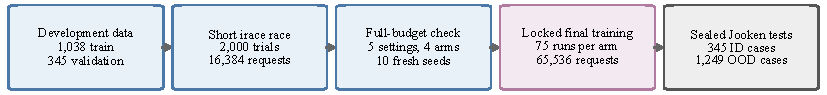
\includegraphics[width=0.75\textwidth]{fig01.pdf}
\caption{Separation of development, configuration, final training, and locked evaluation. The outer irace procedure sees validation costs; the inner GEP search sees only its assigned training cases. Hyperparameters are fixed before any ID, OOD, row-permutation, or transfer score is used.}
\label{fig:Flow}
\end{figure*}

The run count was power-informed rather than copied from a 30-run convention. A pilot-paired standard deviation of 2,192$\ppm$ and a smallest effect of interest of 872$\ppm$ implied about 67 paired runs for 80\% power under the planned multiplicity; 75 leaves a small failure margin. Every arm uses the same master-seed indices and random-stream keys. A common tuned setup keeps the ablation focused on the available terminals.

The predeclared primary contrast is FULL minus BASE on the 345-case ID test. A crossed hierarchical bootstrap resamples 75 seed blocks and 115 sibling-group blocks together for 10,000 replicates. Equivalence requires the entire 90\% interval to lie within the declared $\pm872\ppm$ margin (two one-sided tests at $\alpha=0.05$). Secondary FULL-minus-CAP and FULL-minus-SCALE contrasts are multiplicity-controlled. The eight-method comparison averages stochastic runs inside each sibling group, uses a blocked Friedman test, and applies Holm-adjusted paired tests against FULL. Error bars for GEP in Fig.~\ref{fig:Headline} resample seeds and groups; fixed-rule bars resample groups only. We do not use overlap between individual error bars to test significance.

Before test evaluation, a machine-readable lock recorded the split, folds, seeds, selected setup, source hashes, contrast family, and figure definitions. The evaluation command refused a hash mismatch. Final runs never stopped early, and cached duplicate expressions still counted against the raw request budget. We retained checkpoints at 1,872, 4,096, 16,384, 21,280, 32,768, and 65,536 requests, along with unique-expression and timing counts. Separate random streams controlled initialization, selection, crossover, and mutation. These details treat seeds, instances, parameters, and artifacts as distinct experimental factors, following reproducibility guidance for evolutionary computation~\cite{repro2021}.


In a separate revision-stage comparison, we reimplemented the kNN selector~\cite{zarate2025} under this Jooken protocol. R class::knn uses $k=1$ and Euclidean distance on mean/max profit, mean/max weight, and $(\rho_{p,w}+1)/2$, computed once per instance. Undefined correlation maps to 0.5. Labels maximize packed profit on the same 1,383 development cases; ties follow DEF, MAXP, MAXPW, MINW. Unlike the published class-balanced synthetic training set, we retain the Jooken distribution. All nearest-distance ties vote; tied class votes use seed 20261021 with fixed instance order. Before new evaluation, we froze source/input hashes, the four previously selected genes, and the protocol; no tuning or GEP retraining was added. We evaluate all nine methods on 345 ID and 1,249 OOD cases. Four formula-minus-kNN ID contrasts resample the 115 sibling groups 10,000 times (seed 20261022), with Bonferroni-adjusted 98.75\% intervals, conditional on these selected models.

\section{Results}
\label{sec:Results}

\subsection{Held-out Quality and Terminal Ablation}

\begin{figure*}[htb!]
\centering
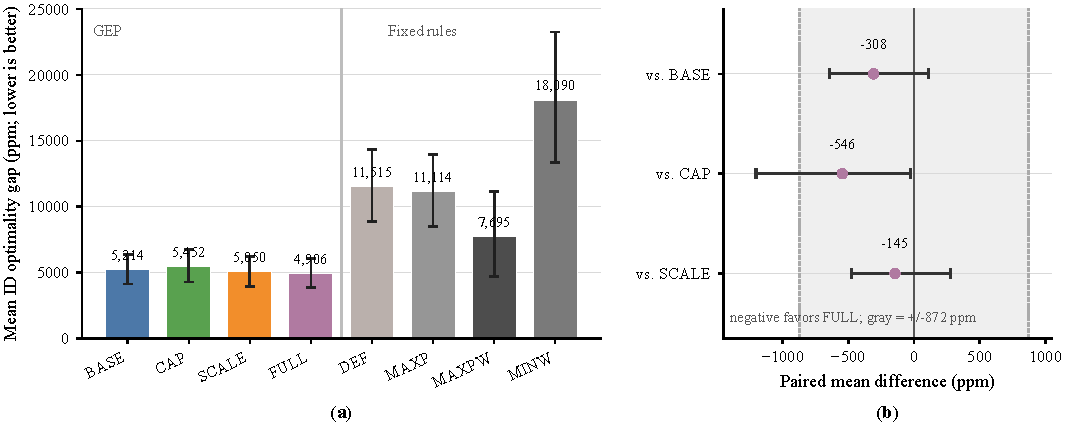
\includegraphics[width=0.75\textwidth]{fig02.pdf}
\caption{Locked ID results. (a) Mean gaps with 95\% hierarchical-bootstrap intervals for 75 GEP runs and group-bootstrap intervals for fixed rules. (b) Paired 95\% intervals for the predeclared terminal contrasts; the gray region marks the practical-equivalence range.}
\label{fig:Headline}
\end{figure*}

All four GEP arms had lower mean ID gaps than the fixed rules in Fig.~\ref{fig:Headline}(a). FULL closed 36.3\% of MAXPW's residual gap; the blocked comparison remained significant after Holm correction ($p=0.0051$). Yet the group difference had mean -2,789.7$\ppm$ and median +83.3$\ppm$, with only 27 wins against 88 losses. Fewer large improvements drove the mean; the exact-solution and tail metrics in Table~\ref{table:Secondary} show that this is not instance-wise dominance.

\begin{table}[htb!]
\caption{Secondary ID metrics. Gaps are in ppm; CVaR$_{.90}$ is the mean gap in the worst 10\% of cases.}
\label{table:Secondary}
\centering
%\setlength{\tabcolsep}{3.3pt}
\begin{tabular}{rrrrr}
\toprule
\textbf{Method} & \textbf{Mean} & \textbf{Median} & \textbf{CVaR$_{.90}$} & \textbf{Exact \%} \\
\midrule
BASE  & 5,214  & 1,497 & 22,897 & 3.64 \\
CAP   & 5,452  & 1,265 & 27,870 & 5.22 \\
SCALE & 5,050  & 1,371 & 22,784 & 9.09 \\
FULL  & 4,906  & 1,118 & 24,234 & 10.67 \\
DEF   & 11,515 & 4,648 & 47,655 & 0.00 \\
MAXP  & 11,114 & 4,563 & 47,565 & 25.22 \\
MAXPW & 7,695  & 78    & 58,548 & 4.93 \\
MINW  & 18,090 & 4,886 & 87,773 & 0.00 \\
\bottomrule
\end{tabular}
\end{table}

MAXPW's small median and large worst-decile mean contrast with FULL's better tail control. MAXP achieves the highest exact-solution rate despite its larger mean gap.

The locked FULL-minus-BASE effect was $-308.2\ppm$, with 95\% interval $[-640.4,112.7]\ppm$ ($p=0.1216$). The 90\% interval $[-589.5,28.4]\ppm$ lies inside $\pm872\ppm$, establishing practical equivalence; FULL was also equivalent to SCALE. FULL minus CAP was -546.4$\ppm$, with 95\% interval $[-1,203.4,-28.3]\ppm$. Overall, the terminal ablation supports the simpler BASE representation rather than a consistent benefit from additional inputs.

Matched random-gene search helps separate evolution from alphabet size. On ID, GEP reduced mean gap relative to its matched random control by 534$\ppm$ for BASE, 655$\ppm$ for CAP, 583$\ppm$ for SCALE, and 1,148$\ppm$ for FULL; all four paired intervals excluded zero. Evolution therefore contributed beyond drawing valid expressions from each alphabet. Only 10 of the 300 GEP models were ranking-equivalent to MAXPW on the fixed probes~(eight CAP and two FULL), so most runs did not merely rediscover the density order.

Table~\ref{table:Expressions} shows one rule per arm. Selection used development data only: among models within one group-level standard error of the best train-plus-validation mean, we chose the shortest expressed region and then a fixed lexical and seed tie-break. These are executable forms, not symbolic claims that protected division behaves like ordinary division at zero.

\begin{table}[htb!]
\caption{Previously development-selected rules and revision comparators. ID means are for individual rules.}
\label{table:Expressions}
\centering
%\setlength{\tabcolsep}{3.5pt}
\begin{tabular}{rlr}
\toprule
\textbf{Rule} & \textbf{Item score} & \textbf{ID ppm} \\
\midrule
BASE-020 & $\pdiv(W,P^2-P)+P(O+2W)$ & 3,705 \\
CAP-008 & $W-\pdiv(W,(1-P)(K+P))$ & 3,657 \\
SCALE-042 & $\pdiv(\pdiv(W,PL)-O,2W-1)$ & 4,404 \\
FULL-071 & $\pdiv(1-2\pdiv(K,P),(1-L)(P+T))$ & 3,306 \\
MAXPW & $p_i/w_i$ & 7,695 \\
kNN & Selected fixed rule & 7,810 \\
\bottomrule
\end{tabular}
\end{table}

The expressed regions contain 15, 11, 13, and 17 symbols. These individual rules differ from the 75-run averages in Fig.~\ref{fig:Headline}. Their ID differences from kNN are -4,105, -4,153, -3,406, and -4,504$\ppm$ (BASE, CAP, SCALE, FULL); adjusted 98.75\% intervals are $[-7907,-827]$, $[-8446,-494]$, $[-7859,409]$, and $[-8355,-1174]\ppm$. SCALE's interval crosses zero. kNN has a better ID median (47$\ppm$) than every selected formula (782--1,911$\ppm$). Pooled OOD means are 3,640, 3,499, 3,413, and 3,498$\ppm$, versus 8,565 for kNN and 10,192 for MAXPW.

\subsection{Generalization, Budget, and Robustness}
\label{sec:Generalization}

\begin{figure*}[htb!]
\centering
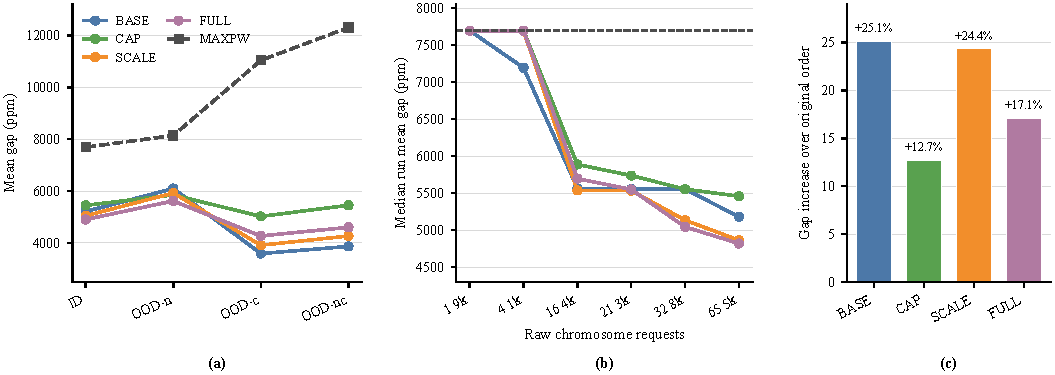
\includegraphics[width=0.75\textwidth]{fig03.pdf}
\caption{Three limits on the headline mean. (a) GEP and MAXPW on locked Jooken regions. (b) Median of the 75 run-level ID means across stored budget checkpoints; the dashed line is MAXPW. (c) Percent change when the canonical order is pooled with ten deterministic row permutations.}
\label{fig:Robustness}
\end{figure*}

Figure~\ref{fig:Robustness}(a) stays within the Jooken generator while changing the item count, capacity, or both. Every GEP arm retained a lower aggregate mean gap than MAXPW in all three OOD regions. For example, FULL scored 5,622$\ppm$ on OOD-$n$, 4,271$\ppm$ on OOD-$c$, and 4,605$\ppm$ on OOD-$nc$, compared with 8,145, 11,042, and 12,311$\ppm$ for MAXPW. This positive extrapolation occurs within one generator, not evidence of a universal knapsack rule.

The budget checkpoints in Fig.~\ref{fig:Robustness}(b) explain why the final study used more search than the pilot. At 1,872 requests, a typical run was close to MAXPW. The largest improvement appeared by 16,384 requests, with smaller but visible gains through 65,536. More computation was useful, but the curve does not make 65,536 a universally optimal budget.

The mathematical problem is invariant to input-row order, but terminal $O$ and the stable tie-break are not. Pooling the original order with ten fixed permutations raised the mean ID gap by 25.1\% for BASE, 12.7\% for CAP, 24.4\% for SCALE, and 17.1\% for FULL. The gain over MAXPW remained useful on average, but the audit limits the claim to the tested representation and decoder.

\subsection{Computation and External Transfer}

On our computer, the irace main race took about 3.6 wall-clock hours. The full-budget survivor check raised complete hyperparameter selection to about 8.5 hours. Final training took 18.4 wall-clock hours; saved run records sum to 62.38 worker-hours because four workers ran concurrently. Numerical-library threads were limited to one per worker. The machine used was a 10-core Apple M2 Pro MacBook Pro with 16 GB RAM. These timings describe reproducibility on one machine, not solution quality.

\begin{table}[htb!]
\caption{Descriptive runtime on our computer. Tuning times are reconstructed from saved timestamps; worker-hours sum concurrent runs.}
\label{table:Runtime}
\centering
%\setlength{\tabcolsep}{4pt}
\begin{tabular}{rrr}
\toprule
\textbf{Stage} & \textbf{Wall h} & \textbf{Worker h} \\
\midrule
Main irace race & 3.60 & 10.14 \\
Full-budget survivors & 4.88 & 18.38 \\
Final training & 18.41 & 62.38 \\
Locked evaluation & 1.18 & ---\\
Unresolved oracle attempt & 1.10 & 4.38 \\
\bottomrule
\end{tabular}
\end{table}

Once frozen, the rules were cheap to reuse relative to training. The complete locked evaluation applied 41.5 million model/method-instance pairs in 1.18 hours, about 9,747 evaluations per second on our machine. This is the central cost trade-off: an evolved rule may amortize its training over many similar cases, but only if it transfers.

The external audit shows why that condition matters. Without retraining, the best GEP arm on the 31,800 Pisinger cases was CAP at 71,782$\ppm$; MAXPW scored 2,812$\ppm$. Every GEP arm was worse than MAXPW in all 13 classes. This result does not test what GEP could learn if trained on Pisinger. It shows only that a Jooken-trained rule should not be presented as a general knapsack rule. The failure therefore does not cancel the held-out Jooken result; it rejects a broader zero-shot claim that this experiment was not designed to support.

\subsection{Discussion}
\label{sec:Discussion}

The original study supports learning compact Jooken rules, while rejecting a meaningful FULL-over-BASE representation benefit. The additional comparison supports lower selected-rule mean gaps than the reimplemented kNN selector for three formulae, conditional on the fixed models and Jooken development distribution. SCALE's interval and kNN's better median prevent a uniform superiority claim.

The mean advantages reflect protection against large gaps, not success on most groups or dominance in exact recovery. Applications prioritizing the median or exact solutions may prefer another rule.

Tuning reduced the risk of an arbitrary setting, but we did not define a formal untuned control. The five full-budget survivors varied in validation quality; their comparison supports the selection procedure, not an exact counterfactual gain from tuning. Validation remains selection data after repeated use.

Limits remain: prior inspection of Jooken, row-order sensitivity, unequal alphabet sizes, and failed zero-shot Pisinger transfer. Retraining on Pisinger or mixed benchmarks needs a separate locked study; these data cannot predict its benefit or whether it would surpass MAXPW.

\section{Conclusion and Future Work}
\label{sec:Conclusion}

GEP evolved inspectable rules with lower held-out mean gaps than four fixed rules on hard Jooken instances, with gains across new parameter levels and over random search. The richer terminals did not meaningfully improve BASE. Three selected formulae also improve mean gap over the revision kNN comparator, under the stated training distribution and conditional inference. Computation cost, order sensitivity, uneven wins, and failed transfer restrict these findings to the tested family.

Future work will study order-invariant representations and decoders, domain-specific and multi-domain training on mixed Jooken/Pisinger benchmarks, and adaptive selection among complementary learned rules under locked evaluation.

\begin{thebibliography}{00}

\bibitem{kellerer2004}
H. Kellerer, U. Pferschy, and D. Pisinger, \emph{Knapsack Problems}.
Berlin, Germany: Springer, 2004, doi: 10.1007/978-3-540-24777-7.

\bibitem{burke2013}
E. K. Burke, M. Gendreau, M. Hyde, G. Kendall, G. Ochoa, E. \"Ozcan,
and R. Qu, ``Hyper-heuristics: A survey of the state of the art,''
\emph{J. Oper. Res. Soc.}, vol. 64, no. 12, pp. 1695--1724, 2013,
doi: 10.1057/jors.2013.71.

\bibitem{ferreira2001}
C. Ferreira, ``Gene expression programming: A new adaptive algorithm for
solving problems,'' \emph{Complex Systems}, vol. 13, no. 2, pp. 87--129,
2001.

\bibitem{drake2014}
J. H. Drake, M. Hyde, K. Ibrahim, and E. \"Ozcan, ``A genetic programming
hyper-heuristic for the multidimensional knapsack problem,'' \emph{Kybernetes},
vol. 43, no. 9/10, pp. 1500--1511, 2014,
doi: 10.1108/K-09-2013-0201.

\bibitem{zarate2025}
J. E. Z\'arate-Aranda and J. C. Ortiz-Bayliss,
``Machine-learning-based hyper-heuristics for solving the knapsack problem,''
\emph{Pattern Recognit. Lett.}, vol. 196, pp. 338--343, 2025,
doi: 10.1016/j.patrec.2025.03.011.

\bibitem{dokeroglu2024}
T. Dokeroglu, T. Kucukyilmaz, and E.-G. Talbi,
``Hyper-heuristics: A survey and taxonomy,''
\emph{Comput. Ind. Eng.}, vol. 187, Art. no. 109815, 2024,
doi: 10.1016/j.cie.2023.109815.

\bibitem{liu2024eoh}
F. Liu \emph{et al.},
``Evolution of heuristics: Towards efficient automatic algorithm
design using large language model,''
in \emph{Proc. 41st Int. Conf. Mach. Learn. (ICML)},
ser. Proceedings of Machine Learning Research, vol. 235,
2024, pp. 32201--32223.

\bibitem{jooken2023mcts}
J. Jooken, P. Leyman, T. Wauters, and P. De Causmaecker,
``Exploring search space trees using an adapted version of Monte Carlo
tree search for combinatorial optimization problems,''
\emph{Comput. Oper. Res.}, vol. 150, Art. no. 106070, 2023,
doi: 10.1016/j.cor.2022.106070.

\bibitem{jooken2022}
J. Jooken, P. Leyman, and P. De Causmaecker, ``A new class of hard problem
instances for the 0--1 knapsack problem,'' \emph{Eur. J. Oper. Res.},
vol. 301, no. 3, pp. 841--854, 2022,
doi: 10.1016/j.ejor.2021.12.009.

\bibitem{pisinger2005}
D. Pisinger, ``Where are the hard knapsack problems?''
\emph{Comput. Oper. Res.}, vol. 32, no. 9, pp. 2271--2284, 2005,
doi: 10.1016/j.cor.2004.03.002.

\bibitem{ortiz2013}
J. C. Ortiz-Bayliss, E. \"Ozcan, A. J. Parkes, and H. Terashima-Mar\'in,
``A genetic programming hyper-heuristic: Turning features into heuristics for
constraint satisfaction,'' in \emph{Proc. UKCI}, 2013, pp. 183--190,
doi: 10.1109/UKCI.2013.6651304.

\bibitem{irace2016}
M. L\'opez-Ib\'a\~nez, J. Dubois-Lacoste, L. P\'erez C\'aceres, T. St\"utzle,
and M. Birattari, ``The irace package: Iterated racing for automatic algorithm
configuration,'' \emph{Oper. Res. Perspect.}, vol. 3, pp. 43--58, 2016,
doi: 10.1016/j.orp.2016.09.002.

\bibitem{repro2021}
M. L\'opez-Ib\'a\~nez, J. Branke, and L. Paquete, ``Reproducibility in
evolutionary computation,'' \emph{ACM Trans. Evol. Learn. Optim.}, vol. 1,
no. 4, Art. no. 14, pp. 1--21, 2021, doi: 10.1145/3466624.

\end{thebibliography}

\end{document}
